% !TEX TS-program = pdflatex
% !TEX encoding = UTF-8 Unicode

% This is a simple template for a LaTeX document using the "article" class.
% See "book", "report", "letter" for other types of document.

\documentclass[11pt]{article} % use larger type; default would be 10pt

\usepackage[utf8]{inputenc} % set input encoding (not needed with XeLaTeX)
%\usepackage{babel}
%%% Examples of Article customizations
% These packages are optional, depending whether you want the features they provide.
% See the LaTeX Companion or other references for full information.

%%% PAGE DIMENSIONS
\usepackage{geometry} % to change the page dimensions
\geometry{a4paper} % or letterpaper (US) or a5paper or....
% \geometry{margin=2in} % for example, change the margins to 2 inches all round
% \geometry{landscape} % set up the page for landscape
%   read geometry.pdf for detailed page layout information

\usepackage{graphicx} % support the \includegraphics command and options

% \usepackage[parfill]{parskip} % Activate to begin paragraphs with an empty line rather than an indent

%%% PACKAGES
\usepackage{booktabs} % for much better looking tables
\usepackage{array} % for better arrays (eg matrices) in maths
\usepackage{paralist} % very flexible & customisable lists (eg. enumerate/itemize, etc.)
\usepackage{verbatim} % adds environment for commenting out blocks of text & for better verbatim
\usepackage{subfig} % make it possible to include more than one captioned figure/table in a single float
\usepackage{setspace} %paquete para interlineado
\usepackage{graphicx} %para insertar graficos
\usepackage{parskip} % npi de q es
\usepackage{color} %colores
\usepackage{float}


% These packages are all incorporated in the memoir class to one degree or another...

%%% HEADERS & FOOTERS
\usepackage{fancyhdr} % This should be set AFTER setting up the page geometry
\pagestyle{fancy} % options: empty , plain , fancy
\renewcommand{\headrulewidth}{0pt} % customise the layout...
\lhead{}\chead{}\rhead{}
\lfoot{}\cfoot{\thepage}\rfoot{}

%%% SECTION TITLE APPEARANCE
\usepackage{sectsty}
\allsectionsfont{\sffamily\mdseries\upshape} % (See the fntguide.pdf for font help)
% (This matches ConTeXt defaults)

%%% ToC (table of contents) APPEARANCE
\usepackage[nottoc,notlof,notlot]{tocbibind} % Put the bibliography in the ToC
\usepackage[titles,subfigure]{tocloft} % Alter the style of the Table of Contents
\renewcommand{\cftsecfont}{\rmfamily\mdseries\upshape}
\renewcommand{\cftsecpagefont}{\rmfamily\mdseries\upshape} % No bold!

%%% END Article customizations

\usepackage[spanish]{babel}
\usepackage{listings} 
%%% The "real" document content comes below...

\title{Proyecto de Lenguajes de Programaci\'on \\ Primer Parcial}
\author{\\Fausto Mora \\Christian Vergara \\ Angel Gonz\'alez}
%\date{} % Activate to display a given date or no date (if empty),
         % otherwise the current date is printed 
\begin{document}


%\date{} % Activate to display a given date or no date (if empty),
         % otherwise the current date is printed 

\maketitle

\newpage
\thispagestyle{empty}
\tableofcontents

\newpage
\thispagestyle{empty}


\section{Introducción}

\section{Descripci\'on del Proyecto}
\subsection{Prop\'osito}
Al finalizar el proyecto, los responsables del mismo presentaremos una aplicaci\'on para dispositivos m\'oviles para la plataforma Android; desarrollado haciendo uso del entorno de desarrollo Eclipse, y de herramientas de software y dispositivos en donde pueda ser emulado y ejecutado, a fin de adquirir conocimientos en dicho lenguaje de programaci\'on y las herramientas involucradas, para fortalecer nuestras competencias en el "Desarrollo de proyectos con diferentes lenguajes de programaci\'on representando diferentes paradigmas de lenguajes."
\subsection{Producto}
La aplicaci\'on desarrollada corresponde al juego \textsl{Buscaminas} del sistema Windows. El juego será ejecutable en distintos dispositivos que soporten el sistema Andorid, teniendo preferencia en los dispositivos m\'oviles de pantalla grande ( para un mejor uso de la aplicaci\'on).
\\El producto ser\'a desarrollado en el entorno Eclipse disponiendo del SDK para Android. El juego ser\'a emulado en el software haciendo uso del software Genymotion y podr\'a ser ejecutado en dispositivos Android con un API desde la versi\'on 2.1 (Dependiendo de la disponibilidad de componentes presentes en dicho API y que sean usados en nuestro proyecto), hasta las versiones de Andorid m\'as recientes.
\subsection{Objetivos}
Para lograr cumplir nuestro prop\'osito planteamos los siguientes objetivos.
\subsubsection{Objetivos Generales}
\begin{itemize}
\item Desarrollar una Aplicaci\'on para el sistema Android.
\item Conocer la sintaxis y sem\'antica del lenguaje de programaci\'on de la platarforma Android.
\item Desarrollar competencias en la utilizaci\'on de diferentes paradigmas de los lenguajes de programaci\'on.
\end{itemize}
\subsubsection{Objetivos Espec\'ificos}
\begin{itemize}
\item Implementar el juego Buscaminas del sistema Windows respetando todas sus funcionalidades.
\item Hacer uso de herramientas que nos permitan desarrollar aplicaciones para dispositivos m\'oviles.
\item Utilizar las caracter\'isticas del lenguaje de programac\'on Android de manera eficiente y \'optima.
\end{itemize}
\subsection{Alcance}
\subsubsection{Caracter\' isticas implementadas}
El \'area para la que esta desarrollado nuestro proyecto es la de dispositivos m\'oviles.
La aplicaci\'on desarrollada posee caracter\'isticas muy similares al juego Buscaminas de Windows y a continuaci\'on se mencionan las caracter\'isticas implementadas en en plazo de realizaci\'on del proyecto.
\\La aplicaci\'on consta de una pantalla principal  donde se presenta al usuario las siguientes opciones: Iniciar Juego, Instrucciones, Ranking, Desarrolladores y Salir. Cada opci\'on presentada en la pantalla principal desencadena una actividad diferente al ser seleccionada.
\\Para Iniciar el juego hay que escoger entre las tres dificultades disponibles o la opci\'on Personalizado. Las tres dificultades implementadas son: Principiante, Normal, Experto. En la primera se presenta un tablero de juego de 8 x 8 celdas donde se hallan escondidas 10 minas. En la segunda se presenta un tablero de juego de 16 x 16 celdas donde se hallan escondidas 40 minas. En la tercera se presenta un tablero de juego de 16 x 30 celdas donde se hallan escondidas 99 minas. La opci\'on de juego personalizado le permite al usuario determinar las dimensiones del tablero (n\'umero de celdas por columna y por fila) asi como el n\'umero de minas escondidas en el tablero.
\\Se implemento la manera de asignar minas en el tablero una vez que se haya dado el primer clic en una de las casillas. Esto se realizo\' o con el fin de evitar que el usuario pierda una partida con el primer clic.
\\En la pantalla de juego se incluye un reloj que muestra segundo a segundo el tiempo que transcurre durante el juego. Este reloj inicia su marcha desde el primer clic.
\\Tambi\'en se implemeto un bot\' on de reinicio que permite empezar un nuevo juego en cuanto es presionado. Puede ser usado en cualquier momento.
\\Incorporamos dos botones m\'as a la pantalla de juego.El primero, al ser presionado, permite que el siguiente clic sea para colocar una bandera. El segundo bot\' on, una vez presionado, permite que el siguiente clic sea para quitar una bandera del tablero.
\\Para poder guardar las puntuaciones m\' as sobresalientes que los usuarios logren se hace uso de una base de datos para Android (SQLite). Aqu\' i se almacenan los nombres y puntuaciones de los usuarios que logren ingresar en el ranking.
\subsubsection{Caracter\' isticas no implementadas}
El uso de Drag and Drop no fue implementado para usar banderas en el juego. Consideramos que es m\' as sencillo implementarlo usando botones, pero la principal justificaci\'on para ello es que consideramo que se invierte tanto tiempo en seleccionar un bot\' on y hacer clic sobre una celda que llendo al mismo bot\' on para luego arrastrar su contenido a otra celda.

\subsection{Entregables}
El proyecto incluye la entrega de lo siguiente:

\begin{itemize}
\item El link del repositorio GIT donde se encuentra el c\'odigo fuente.
\item Documentación en LaTeX ( incluidos el PDF y el c\'odigo fuente). Estos documentos y todos los recursos que se necesiten para la ejecuci\'on del c\'odigo fuente deber estar dentro de una carpeta llamada \textsl{doc}.
\item  El proyecto ser\'a presentado en un dispositivo m\'ovil corriendo con todas sus funcionalidades.
\end{itemize}

\subsection{Restricciones}
La principal limitaci\'on de nuestro proyecto se debe al tama\~no de la pantalla del dispositivo en donde se ejecute.
Esto se debe al dise\~no del tablero del juego. Al estar compuesto de celdas y al ser una aplicaci\'on t\'actil se dificulta la jugabilidad en dispositivos de pantalla peque\~na.
Es por esta raz\'on que es preferible ejecutar la aplicaci\'on en dispositivos de pantalla grande.

\newpage
\thispagestyle{empty}

\section{Diagramas de casos de uso }

\begin{center}

	\begin{figure}[h!]
  		\centering
    		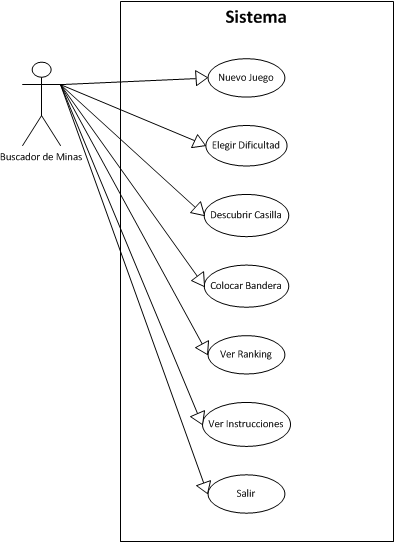
\includegraphics[width=0.7\textwidth]{imagenes/casosdeusos.png}
  		\caption{Casos de Usos}
		\label{fig:casosdeusos}
	\end{figure}
\end{center}

\newpage
\thispagestyle{empty}

\section{Diagrama de clases }

\begin{center}

	\begin{figure}[h!]
  		\centering
    		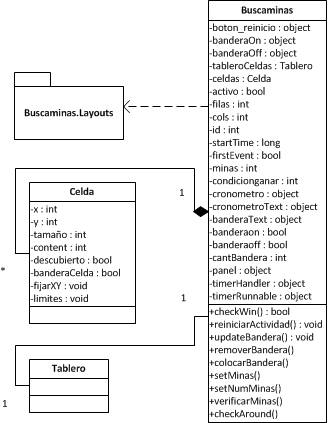
\includegraphics[width=0.7\textwidth]{imagenes/diagramaClases.jpg}
  		\caption{Diagrama de Clases}
		\label{fig:diagclases}
	\end{figure}
\end{center}

\newpage
\thispagestyle{empty}

\section{Conclusiones}


\end{document}
